\documentclass{article}
\usepackage{multicol}
\usepackage[utf8]{inputenc}
\usepackage{graphicx}
\usepackage{geometry}
\usepackage{lscape}
\PassOptionsToPackage{hyphens}{url}\usepackage{hyperref}
 \geometry{
 a4paper,
 left=20mm,
 right=20mm
 }

\DeclareGraphicsExtensions{.png,.pdf}

\title{\vspace{-2cm}Screws Manual}
\date{}
\begin{document}
\begin{landscape}
\maketitle

\vspace{-1cm}

Last updated: \today


\begin{center}
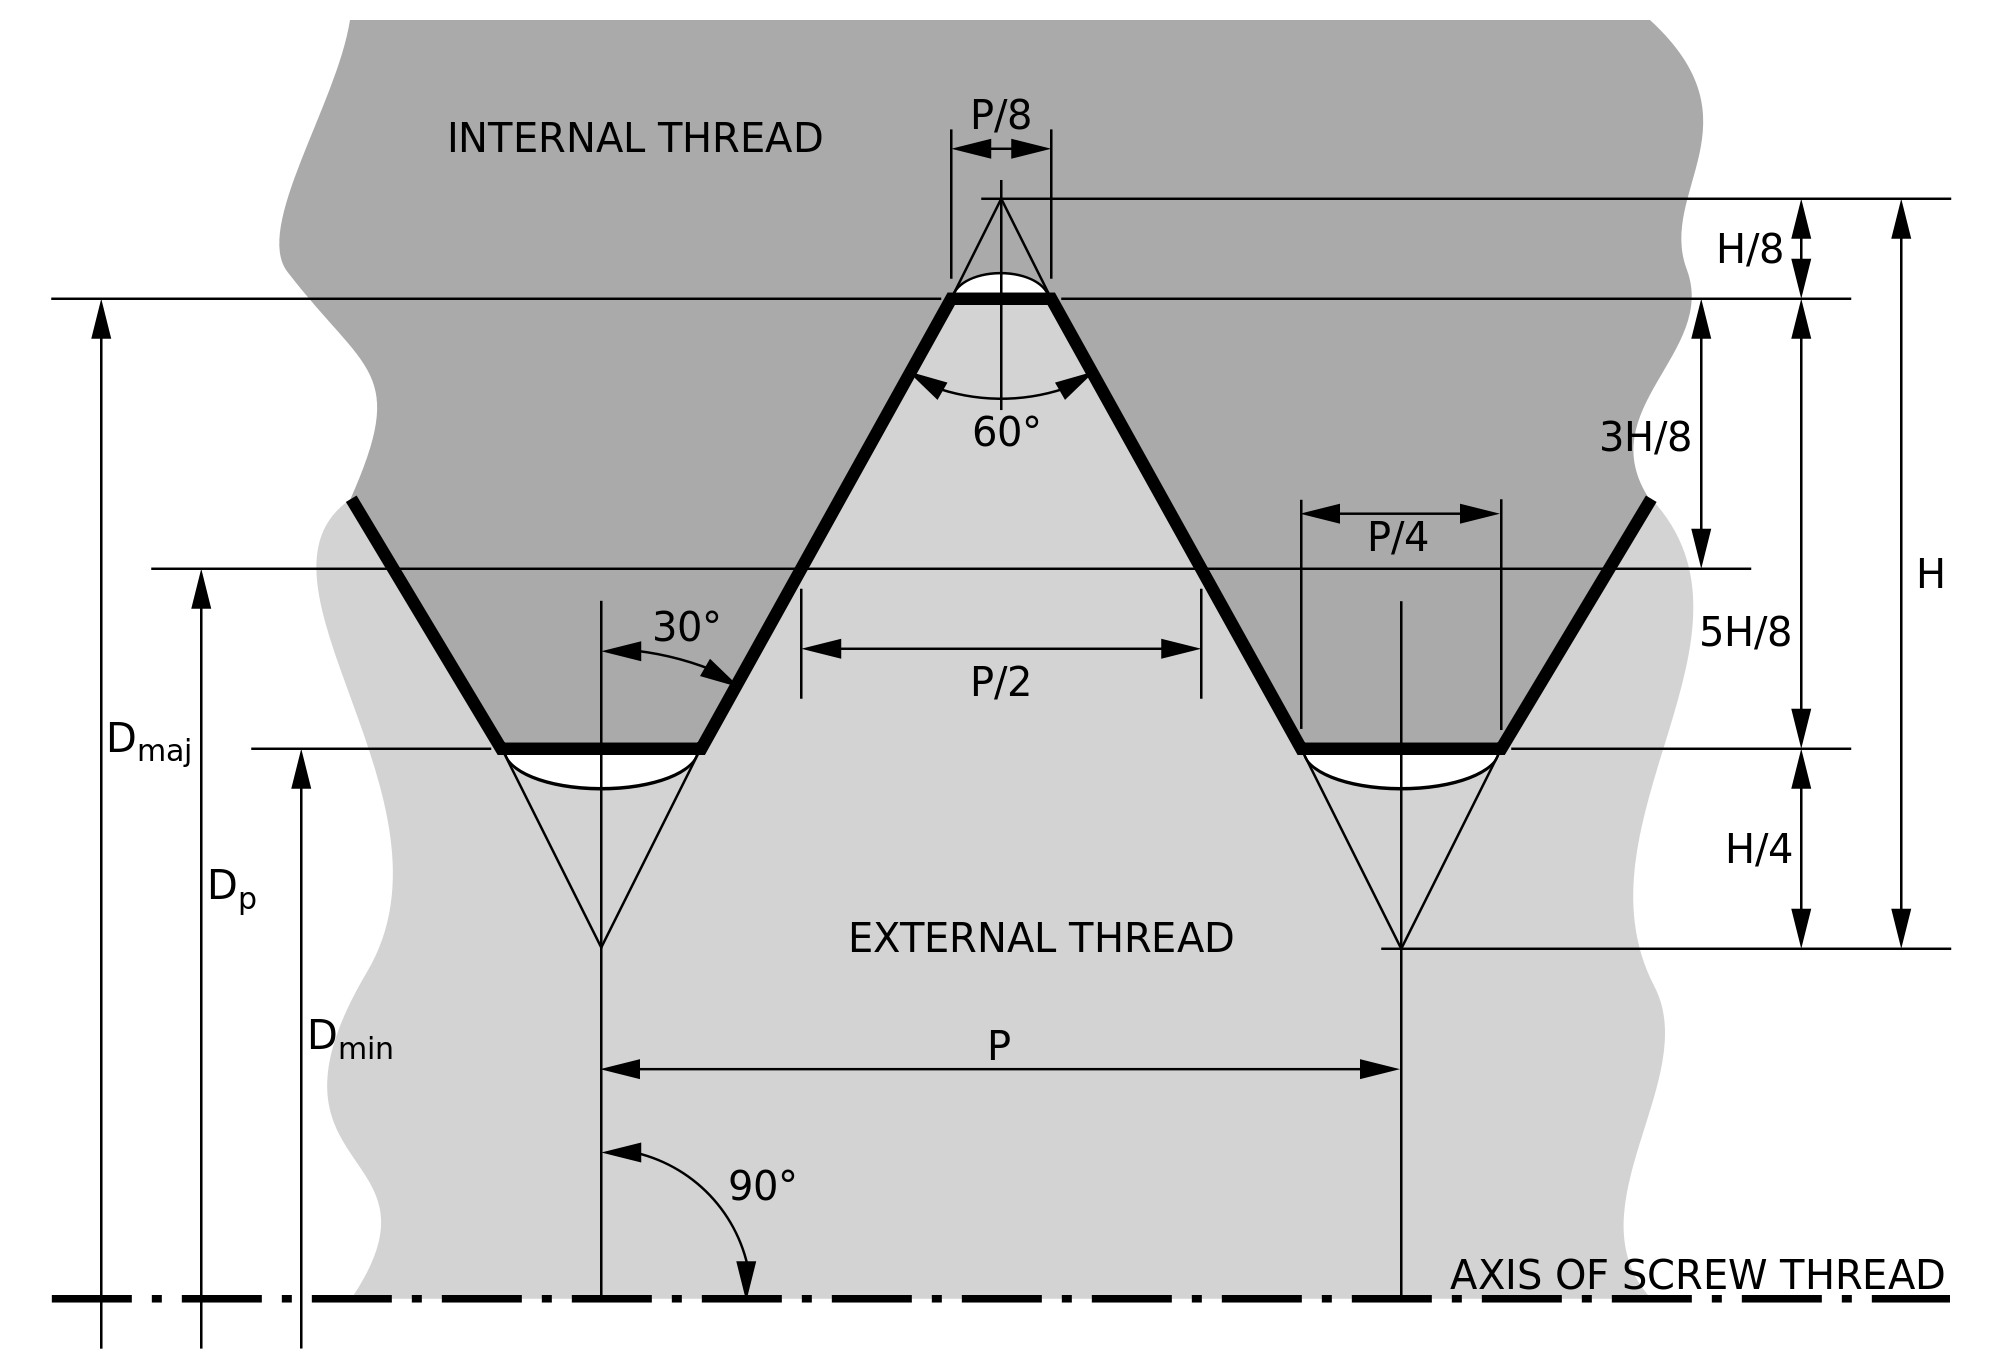
\includegraphics[width=20cm]{assets/screws.png}\\
Image from WikiCommons
%
\end{center}
\end{landscape}

\begin{multicols}{2}

\section{Brief description}

\begin{enumerate}
  \item $H$ is the height of the fundamental screw triangle. You don't actually need to measure this.
  \item $P$ is the pitch, the length of the fundamental screw triangle. use a Vernier Caliper to measure the length of a convenient, integer number of a pitch lengths. Alternatively,
  \item $D$ is the diameter of the screw at various points. The maximum diameter, $D_{major}$ gives you the relevant diameter that is used to reference the screw.,
\end{enumerate}

\section{Naming the screw}

\subsection{Imperial}

Diameter --- Threads per inch --- Length --- Type of screw

e.g. $\frac{1}{4}$''-20 $\frac{5}{8}$'' cap screw

\subsection{Metric}

Diameter --- Pitch --- Length --- Type of screw

e.g. M4x0.7 10mm set screw

\end{multicols}

\section{Imperial Screw Thread Standard}
\begin{tabular}{@{}lllll@{}}
\multicolumn{2}{l}{}Major Pitch Diameter $D$ (inch / mm) & Threads per inch & Preferred cutting tap drill\\
 \#0 & 0.0600 / 1.5240  & None & None \\
 \#1 &  &  &  \\
 \#2 &  &  &  \\

\end{tabular}


\section{Metric Screw Thread Standard}

\begin{tabular}{@{}llll@{}}
 Major diameter $D$/mm & Pitch $P$/mm & Major Diameter $D$/mm & Pitch $P$/mm \\
 1 & 0.25 & 12 & 1.75 \\
 1.2 & 0.25 & 16 & 2 \\
 1.6 & 0.35 & 20 & 2,5\\
 2 & 0.4 & 24 & 3 \\
 2.5 & 0.45 & 30 & 3.5\\
 3 & 0.5 & 36 & 4\\
 4 & 0.7 & 42 & 4.5\\
 5 & 0.8 & 48 & 5 \\
 6 & 1 & 56 & 5.5 \\
 8 & 1.25 & 64 & 6 \\
 10 & 1.5
\end{tabular}



\end{document}
